\chapter{实验分析}
\label{chapter:evaluation}
本章将对前文中设计并实现的IMS资源映射优化系统进行实验分析和性能测试。我们首先对使用的实验平台和实验环境进行详细的介绍,然后针对每一种具体的实验方案进行展开说明,包括进行实验数据归纳和分析。最后,对实验的总体效果和系统的实际收益进行总结。

\section{实验平台和测试环境}
实验中主要使用了一台浪潮英信大通量标准通用服务器,将其作为虚拟化平台,支持虚拟机的创建、运行和销毁。该测试服务器配置有4颗8核2.13GHz的Intel Xeon至强 E7-4830 CPU,以及128G大小的DDR3内存,并且配有1T容量的标准容量SATA磁盘作为外部储存设备。为了真实考察所设计的系统在实际生产环境中所能达到的实际优化效果,实验测试的进行均在真实的实验室网络环境中,而运行的NFV应用为真实的IP多媒体子系统 Clearwater,可以提供语音视频通话业务。在软件配置方面,宿主机上安装的是7.3版本的CentOS Linux操作系统,使用系统自带的KVM作为虚拟化监视器,所有的虚拟机均安装的14.04版本的Ubuntu操作系统。除了NFV服务自身的软件栈,系统中没有安装运行其他多余的软件,以排除不必要的软件因素的干扰并且将系统运行时的额外性能损失降到最低。在优化系统的具体运行参数选择上,考虑到实际的Clearwater应用我们将优化模型中的带宽调节参数$\alpha$设为0.2,延迟调节参数$\beta$设为0.8;而对于收益函数中的$\theta$和$\delta$,分别为$10^{6}$和0.001。实验所用服务器的具体配置参数如表 \ref{tab:configure} 所示。

\begin{table}[htb]
	\centering
	\bicaption[tab:configure]{实验平台配置参数表}{实验平台配置参数表}{Table}{Table of Testing Environment Configuration}
	\begin{tabular}{ | l | p{9cm} |}\hline
		\textbf{项目} &							 \textbf{配置}  				\\ 	\hline
		服务器        &					 浪潮 NF8560M2, 4节点NUMA架构\\ \hline
		处理器 	   &  Intel Xeon CPU E7-4830,2.13GHz x 4  \\ \hline
		缓存    & 24M L3, 256K L2,  64K L1 \\ \hline
		内存 			&  每个节点32GB DDR3,  共128G   \\   \hline
		硬盘     & 				1 TB SATA disk \\ \hline
		操作系统    & Hypervisor CentOS Linux 7.3, Virtual Machine Ubuntu 14.04 \\ \hline
	\end{tabular}
\end{table}
\newpage

从测试工具及实验手段的角度来说,本章中主要使用了Clearwater平台自带的压力测试工具和主流的性能测试和评估工具:Ping、iPerf\footnote{https://iperf.fr/}和ApacheBench\footnote{http://httpd.apache.org/}。从具体的业务性能到通用的性能测试两个层次进行了深入、翔实的实验。从实验对象上来说,主要的实验集中在对系统网络性能的测试和评估上。从实验目的上来说,本章的实验设计主要从服务链的具体业务和通用网络性能两方面出发,分别对本文所提出的系统进行了测试。实验内容包括:(1)Clearwater压力测试工具的性能测试对比。(2)Ping、iPerf、ApacheBench工具的性能测试对比。

\begin{figure}[!htp]
	\centering
	\subfigure[离散分布]{
		\label{dis:scattering}
		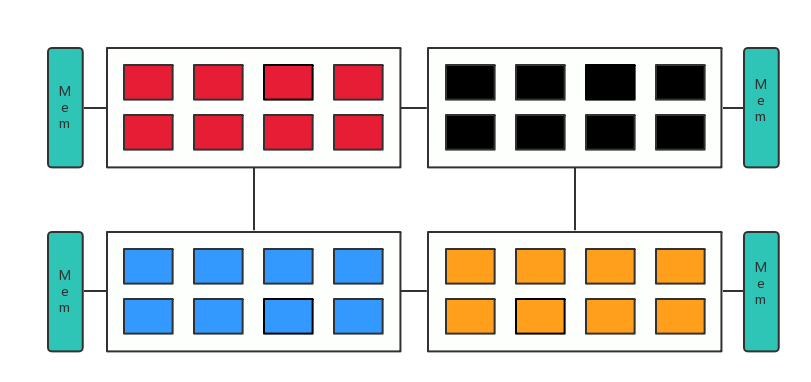
\includegraphics[width=0.7\textwidth]{distribution/Scattering.png}
	}
	\subfigure[聚合分布]{
		\label{dis:uniform}
		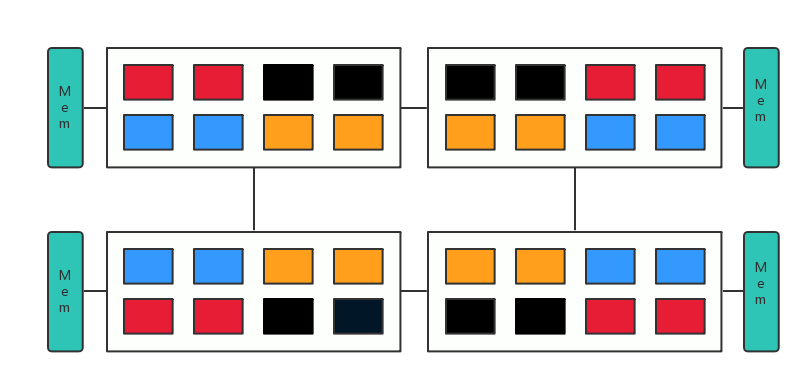
\includegraphics[width=0.7\textwidth]{distribution/Uniform.png}
	}
	\subfigure[随机分布]{
		\label{dis:random}
		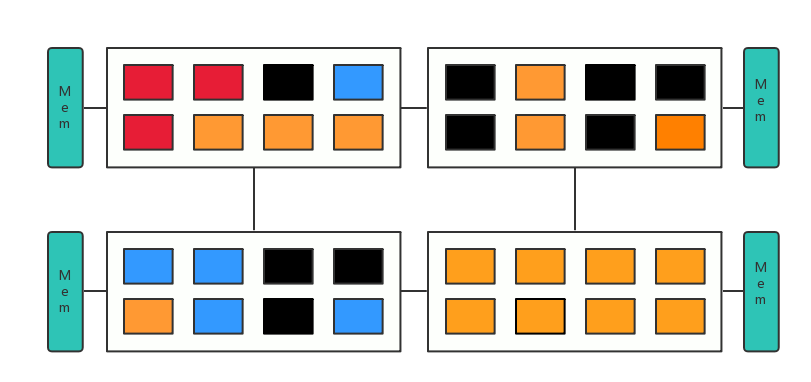
\includegraphics[width=0.7\textwidth]{distribution/Random.png}
	}
	\bicaption[fig:resource]{实例资源分布示意图}{实例资源分布示意图}{Fig}{Resource Distribution Overview}
\end{figure}

除了使用以上所述的测试工具,本文充分考虑了在实际环境下各种网络功能实例在多核物理机上的分布情况,故本文列举了三种可能的实例分布方式如图 \ref{fig:resource}所示,分别为离散分布(图\ref{dis:scattering}所示)、随机分布(图\ref{dis:random}所示)和聚合分布(图\ref{dis:uniform}所示)。图中以不同的色块来代表不同的网络功能,以实例所绑定的物理CPU来代表某个实例的物理资源分配情况。可以看出,在离散分布的情形下,相同的虚拟网络功能实例聚集在同一个处理器节点中,在这样的资源分布下,所有虚拟机实例间具有相近的物理资源数据传输性能。在聚合分布下,每个处理器节点上都被均匀地绑定了实现网络服务链的所有功能实例。而在随机分布的情形下,所有的网络功能实例以随机的方式绑定在所有的物理CPU上。所有本文后续的所有测试将覆盖这三种资源分布,以检验本设计系统在实际应用场景下的有效性。

\section{Clearwater压力测试实验}
本文以按照分布式的方式在配置如表\ref{tab:configure}所示的大通量标准服务器中部署了Clearwater所需的所有功能节点,以KVM作为Hypervisor,所有虚拟机均配置了单个虚拟核、1G的运行内存和10G的磁盘容量,并利用Virtio的网络虚拟化方式提供虚拟网卡。测试负载方面,本文使用了Clearwater平台所提供的测试工具集,选择了其中的标准语音通信业务中用户注册-解注册业务\textit{reg-dereg}作为本文的测试负载。一次\textit{reg-dereg}服务由三个请求组成,分别为:注册请求、认证请求和注销请求。其中任意一个请求一旦超过了最大返回等待时间(10s),则该次请求失败。为了测试系统默认随机策略的性能,我们设定每次实验指定运行300s,运行10次后去平均值作为最终结果。测试工具可以指定不同的初始请求速率来测试不同负载强度下的平均请求响应延迟。使用从发起注册请求到最后一个请求的200回执为止的平均时间作为衡量延迟的具体参数,单位为毫秒。最后以平均的延迟时间和请求的成功率来作为性能比较的依据。

压力测试实验结果如图 \ref{exp:clearwater} 所示,本文测试了在light (50),light-medium(100),medium(500),heavy(1000) 四种请求速率下默认系统与本设计所实现的系统在性能上的差异,在这四种负载下分别测试了三种不同分布下的性能结果作为对照组。深色的柱状条代表默认的随机映射系统的测试结果,浅色的柱状条代表在本设计优化过后的结果。为了方便比较,本文对数据进行了归一化处理,这样能够比较直观的体现出优化前后的性能对比。根据图 \ref{exp:clearwater}所示,可以看出在四种不同大小的负载下,本设计的系统在离散分布和随机分布中都取得了较好的优化效果,服务的延迟平均有接近40\%的下降,而在聚合分布的情况下,服务在优化前后并没有表现出较大的性能差别。进一步的,对比三种分布下的基准和优化的平均性能,不难发现聚合分布的平均性能最高随机分布次之而离散分布最差,而经过本设计的优化之后,离散和随机分布下的平均延迟均低于聚合分布。这样的测试结果基本上是符合测试结果预期的。

首先,针对离散和随机分布,在默认条件下Clearwater系统会随机的选取实例进行组链,在完全没有考虑资源间的数据传输差异的前提下,所产生服务链就可能会有较大的平均服务延迟,而且由于资源分布的离散程度,不同资源之间的数据传输性能有着不同程度的差异;而在聚合分布下,所有的功能实例之间具有相近的数据传输性能,平均性能比较稳定,可以优化的空间较小,故默认系统和优化后的系统并没有显示出明显的性能差异。综合来看,可以认为本设计的优化系统在离散分布和随机分布的情况下能够有效地提升Clearwater服务的性能,提升物理资源的使用效率。

\begin{figure}[htp]
	\centering
	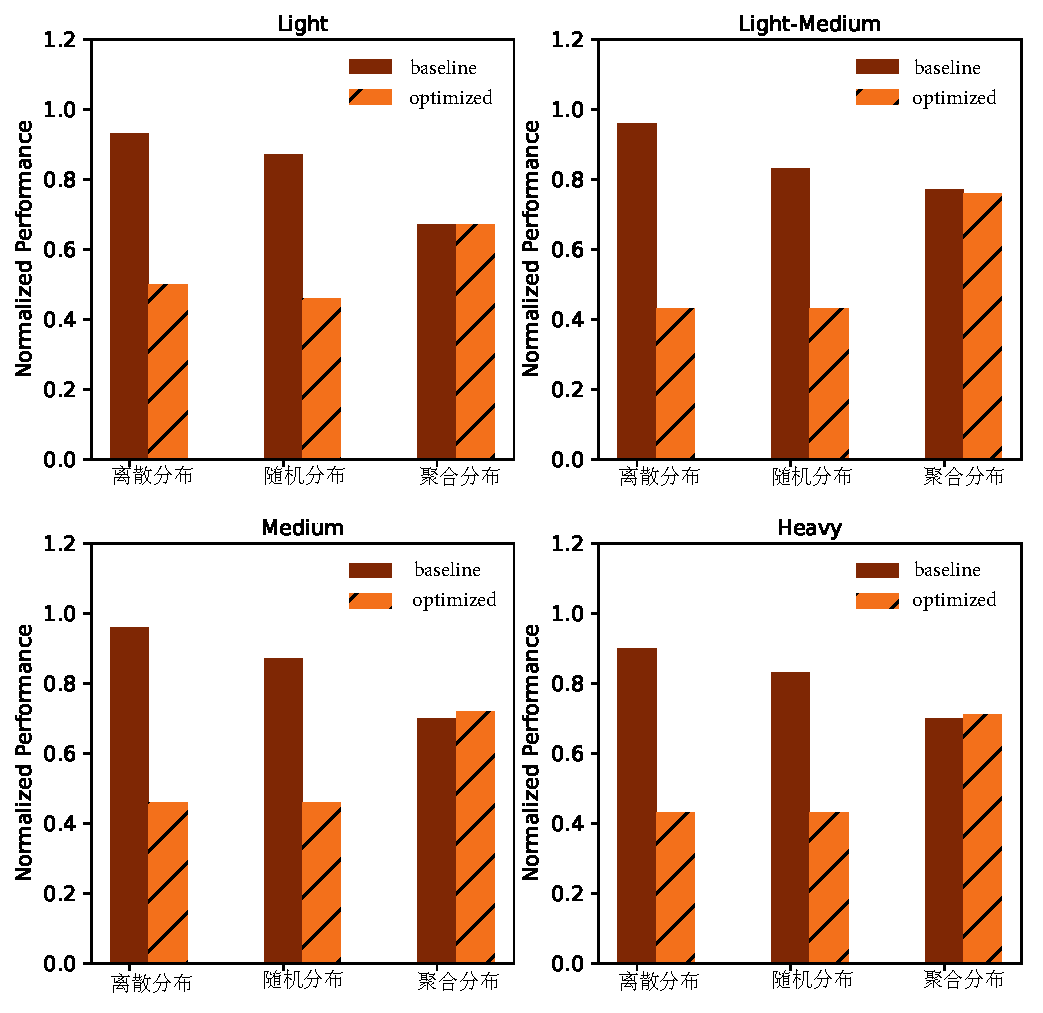
\includegraphics[width=0.8\textwidth]{clearwater1.pdf}
	\bicaption[exp:clearwater]{Clearwater压力测试结果图}{Clearwater压力测试完成时间(越低越快)}{Fig}{Clearwater Stress Performance Test}
\end{figure}
\newpage
\section{网络性能对比实验}
本文除了使用Clearwater自带的压力测试工具测量IMS业务性能之外,也使用了一些测试工具对IMS业务进行模拟测试,用来验证本设计系统的通用性和优化的有效性。为了模拟实际NFV服务的网络功能服务链,本文将优化系统所选择的服务链实例挑选出来与系统随机选择的服务链做对比,分别用Ping,iPerf和ApacheBench来进行端对端的性能测试,并将其结果累计算作服务链的性能结果进行比较和验证优化系统的有效性。同样的,本文测试了在三种不同实例分布下的网络功能服务链映射结果。在性能测试中,本文以默认的随机生成策略的测试结果作为基准数据(Baseline),使用优化后的测试数据(Optimized)进行对比。为了保证数据的可靠性,所有实验均采取多次实验取平均值作为测试结果。

\subsection{Ping实验}
在本小节中,本文使用了轻量级的网络命令Ping来测试系统的累计网络延迟性能。Ping是一个非常轻量级的网络命令,其运行过程中的所引起的CPU和内存额外开销可以忽略不计,因而在网络测试中Ping命令经常被用来测试网络的延迟大小,测试的结果基本与真实网络链路上产生的延迟相等。在本小节的实验中,所有的虚拟机依然采用单个虚拟核、1G运行内存和10G磁盘的配置,测试的虚拟机使用Ubuntu 14.04 Server版本的系统。为了获取服务链累计的延迟信息,本文设置了链路上每一个上游节点都同时向自己相邻的下游节点进行Ping请求,并将每台客户端的测试结果输出并统计。实验所使用的发包时间间隔为0.5秒,测试时间长度为1分钟。
\begin{figure}[!htp]
	\centering
	\subfigure[离散分布下Ping延迟测试(越低越快)]{
		\label{exp:ping_scattering}
		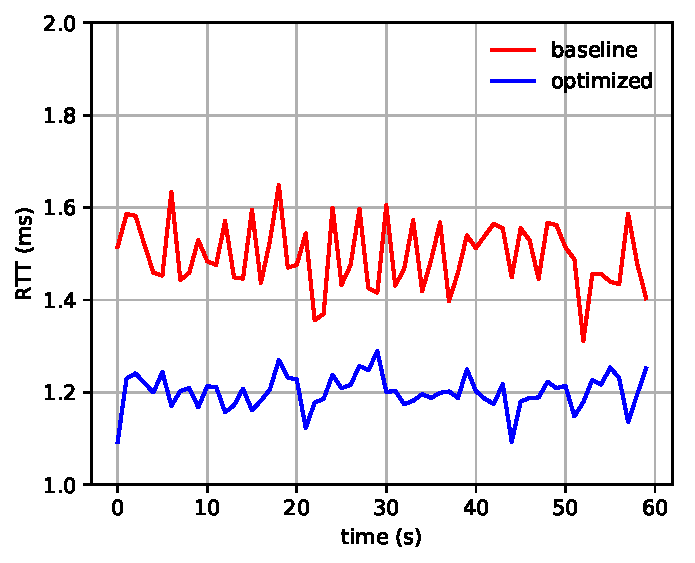
\includegraphics[width=0.70\textwidth]{ping/ping_scattering.pdf}
	}
	\subfigure[聚合分布下Ping延迟测试(越低越快)]{
	\label{exp:ping_uniform}
	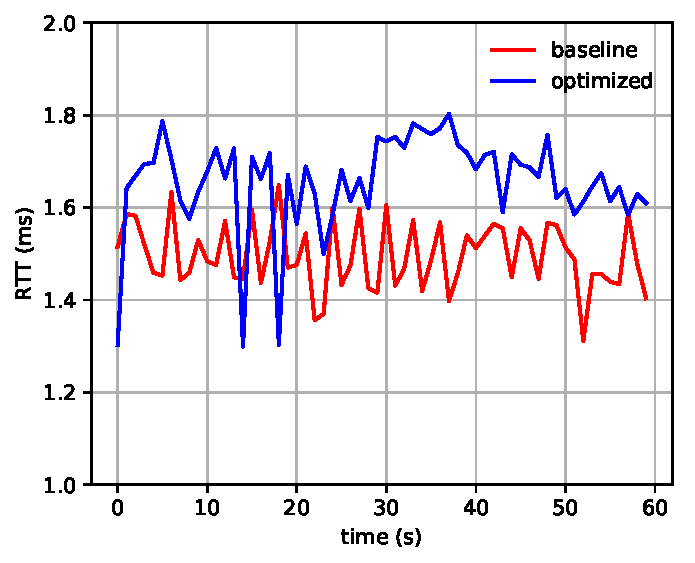
\includegraphics[width=0.70\textwidth]{ping/ping_uniform.pdf}
	}
	\bicaption[exp:ping]{Ping测试结果图}{Ping测试结果图}{Fig}{Ping Test Result}
	
\end{figure}
\begin{figure}
	\addtocounter{subfigure}{2}
	\ContinuedFloat
	\centering
	\subfigure[随机分布下Ping延迟测试(越低越快)]{
	\label{exp:ping_random}
	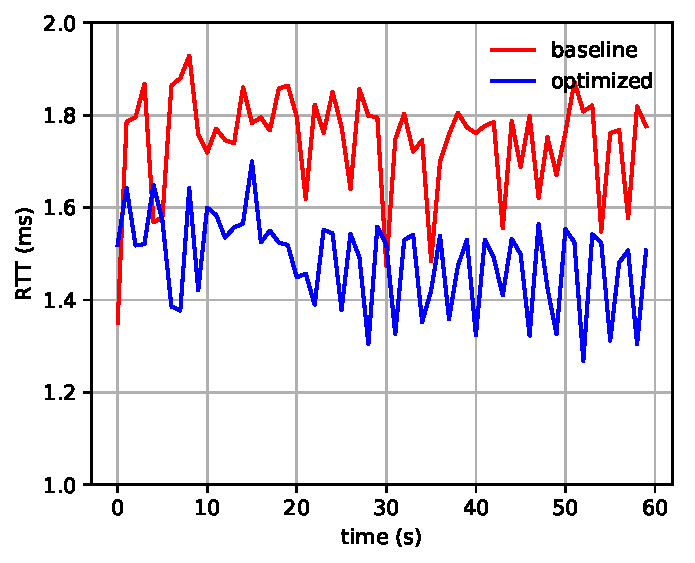
\includegraphics[width=0.70\textwidth]{ping/ping_random.pdf}
	}

	\bicaption[exp:ping]{Ping测试结果图 (续)}{Ping测试结果图 (续)}{Fig}{Ping Test Result (Con't)}
\end{figure}
\newpage
如图 \ref{exp:ping} 所示,红色的折线代表默认的服务链映射策略所选的实例组合所产生的累计延迟,蓝色的折线代表优化系统所选择实例所产生的累计延迟。在统计过程中发现,虽然端到端的Ping测试结果差异比较小,但是当服务链的所有节点的延迟累计起来后,延迟的下降就相对明显了。在离散和随机分布中,如图 \ref{exp:ping_scattering} 和图 \ref{exp:ping_random} 所示,本文观测到了对于每条服务链,都有接近0.2ms的延迟下降,下降的比例接近15\%。而在如图\ref{exp:ping_uniform}聚合分布下,由于所选择的实例间延迟并没有减少,与系统默认的随机策略所选取的实例在数据传输延迟间的差异很小,所以优化前后的性能差异也并不明显。对比三种分布下的延迟数据可以看出,在离散分布的前提下,服务链可以达到最低的累计延迟,相比随机生成的服务链策略有了接近30\%的延迟下降。

\subsection{iPerf实验}
本节中,本文使用iPerf工具来测试系统的网络带宽性能。iPerf是一套可以动态测量基于IP网络的最大执行带宽的测试工具集。它支持调整执行时间、协议和缓冲区大小来进行性能调优。本小节的实验中使用的是更加轻量级的iPerf3来进行测试,测试虚拟机的而配置与Ping实验中的相同。iPerf测试需要手动配置客户端和服务端,因此在所有运行的虚拟机中都配置iPerf服务监听端口,当获取实际链路组合后,以链路上每个前置节点作为客户端向相邻的后置节点发送数据,统计链路上的累计带宽。单次实验的执行时间为30秒,分别使用了数据包大小为1K、4K、16K的测试负载来针对三种不同的实例分布进行了测试,每组实现均执行10次取平均值作为最后的输出结果。
\begin{figure}[!htp]
	\centering
	\subfigure[离散分布下的iPerf吞吐性能(越高越好)]{
		\label{exp:iperf_scattering}
		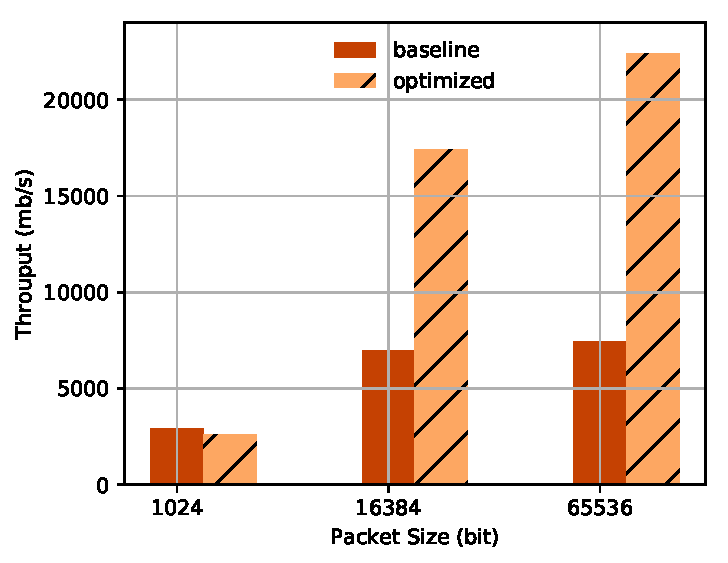
\includegraphics[width=0.70\textwidth]{iperf/iperf_scatter.pdf}
	}
	\subfigure[聚合分布下的iPerf吞吐性能(越高越好)]{
		\label{exp:iperf_uniform}
		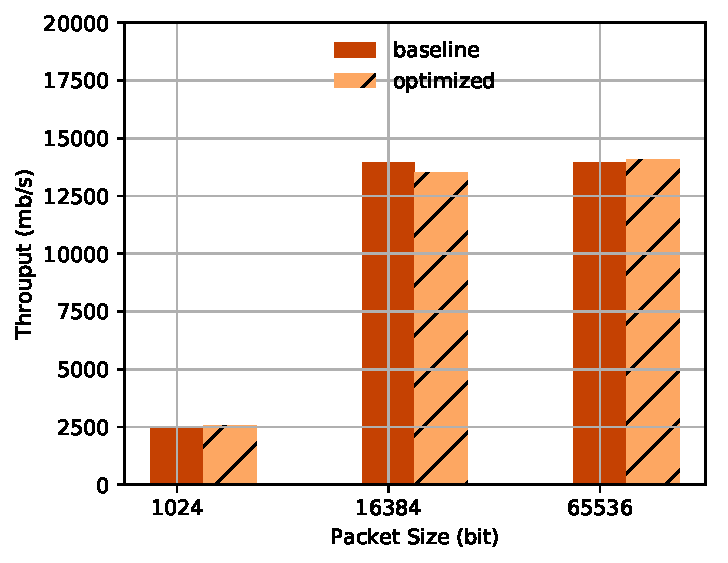
\includegraphics[width=0.70\textwidth]{iperf/iperf_uniform.pdf}
	}
	\bicaption[exp:iPerf]{iPerf测试结果图}{iPerf测试结果图}{Fig}{iPerf Test Result}
\end{figure}
\begin{figure}
	\addtocounter{subfigure}{2}
	\ContinuedFloat
	\centering
	\subfigure[随机分布下的iPerf吞吐性能(越高越好)]{
	\label{exp:iperf_random}
	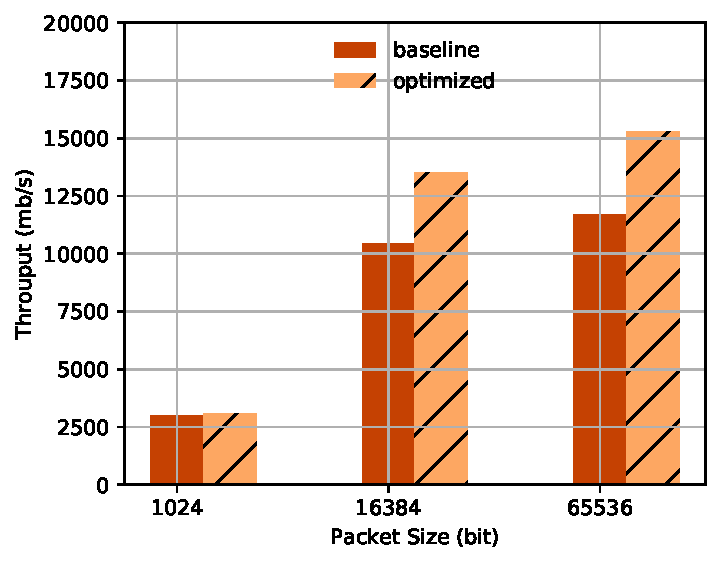
\includegraphics[width=0.70\textwidth]{iperf/iperf_random.pdf}
	}
	\bicaption[exp:iPerf]{iPerf测试结果图 (续)}{iPerf测试结果图 (续)}{Fig}{iPerf Test Result (Con't)}
\end{figure}

如图 \ref{exp:iPerf} 所示,深色柱状条代表默认随机的选取策略所选取的服务链实例组合在iPerf测试场景下的性能测试结果,浅色斜杠条纹柱状条则代表本文优化策略所选取的服务链组合的测试性能测试结果。

通过统计可以发现,在离散分布和随机分布的情况下,服务链的累计带宽有了明显的提升,具体数据如图\ref{exp:iperf_scattering}和图\ref{exp:iperf_random}所示。特别是如图\ref{exp:iperf_scattering}所示,在离散分布的16K大小数据包的测试对照组中,优化后的服务链相比于随机选择的组合,带宽有了接近2倍的提升。但是在1K数据包的测试对照组下,可以发现优化前后的性能变化并不大。通过监测实验时的实时CPU利用率,可以发现当发送1K数据包时,所有的运行实例的CPU接近满负载。结合已知的网络和操作系统知识来分析,在小包的情况下,限制网络带宽的瓶颈在于频繁的数据包处理,数据包数量越多,则CPU处理所需要的开销越高,故在小包情况下,服务链上的资源亲和度并没有对性能有主导影响。而随着数据包大小的提升,可以发现此时各实例之间的资源亲和度的影响逐渐增大,当数据包大小为16K时,更是出现了接近2倍的性能差距。这样的实验结果可以证明本设计系统相比于随机策略的优越性。在离散分布和随机分布下,本设计可以有效地提升服务链的整体网络通信带宽。

同样的,在聚合分布下,如图\ref{exp:iperf_uniform}所示,优化系统并没有体现出优化效果,其原因在于聚合分布下的不同功能实例间具有相近的数据传输性能,所以本文的优化算法与随机策略对比,并没有实质的优化效果。

\newpage
\subsection{ApacheBench实验}
本节中,本文使用ApacheBench来测试在模拟真实业务下NFV服务链的标准性能。ApacheBench是一款用于测量HTTP Web服务器性能的测试工具,最初作为Apache HTTP Server的测试工具,后来被扩展为可以用于测试任何Web服务器。IMS业务纷繁复杂,仅仅使用不同包大小的数据从微观的角度去衡量服务链的性能在实际应用场景下缺乏说服力,所以本节中使用真实的Web服务来测试在真实网络应用场景下的实际性能。在实际应用场景下,业务请求可能包括不同大小不同长度的数据包,在这样的测试场景下进行测试更具有实际意义。ApacheBench的测试原理是由客户单向目标服务器发起资源请求,可以通过命令来创建不同数量的并发访问线程,模拟多个访问者对同一个URL地址进行访问。测试工具会持续访问资源直到完成预先设置的访问总数,并输出每秒所完成的请求次数(rps, requests per second)。本文仿照之前的测试设置,使用了相同的虚拟机配置,在不同映射策略下的虚拟机之间根据服务链数据流的先后关系,进行了累计请求统计。除了不同的实例分布场景这个变量之外,本实验还选择不同请求并发数来考察在不同数据压力负载下的的性能表现,预先设置的访问总数为10万次,每次测试重复10次取平均结果来作为衡量依据。
\begin{figure}[!htp]
	\centering
	\subfigure[离散分布下的Apache Bench吞吐性能(越高越好)]{
		\label{exp:ab_scattering}
		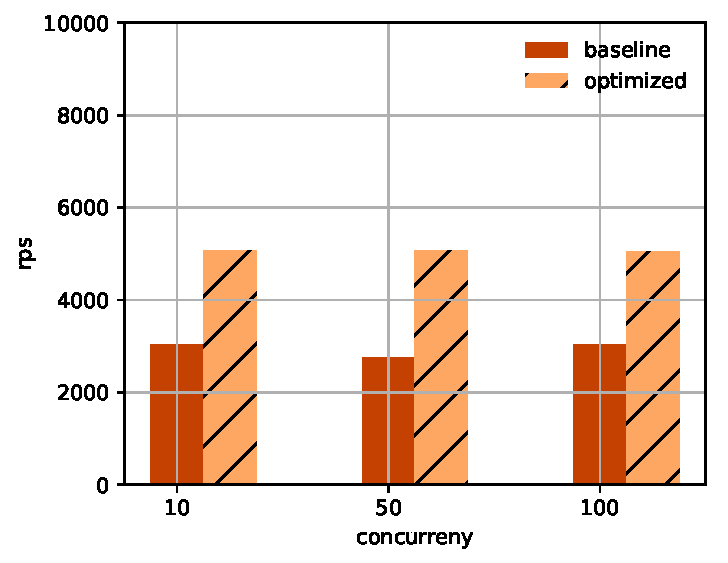
\includegraphics[width=0.70\textwidth]{ab/ab_scatter.pdf}
	}
	\bicaption[exp:ab]{ApacheBench测试结果图}{ApacheBench测试结果图}{Fig}{ApacheBench Test Result}
\end{figure}
\begin{figure}
\addtocounter{subfigure}{1}
\ContinuedFloat
\centering
	\subfigure[聚合分布下的Apache Bench吞吐性能(越高越好)]{
	\label{exp:ab_uniform}
	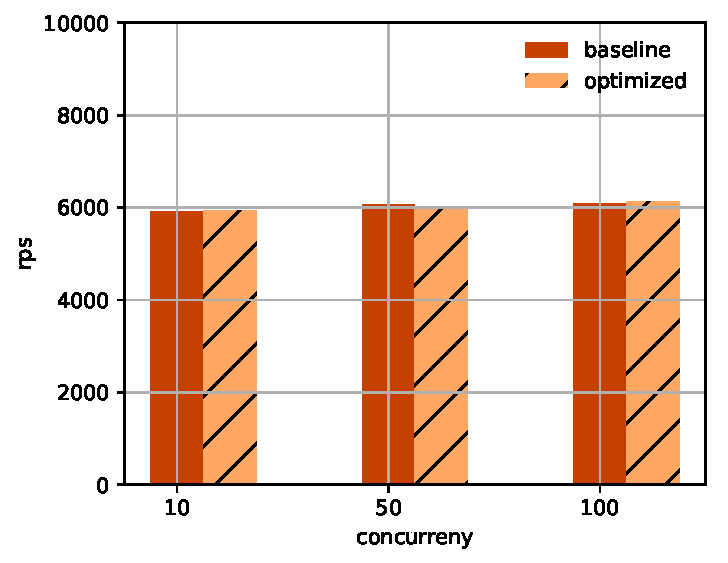
\includegraphics[width=0.70\textwidth]{ab/ab_uniform.pdf}
	}
	\subfigure[随机分布下的Apache Bench吞吐性能(越高越好)]{
	\label{exp:ab_random}
	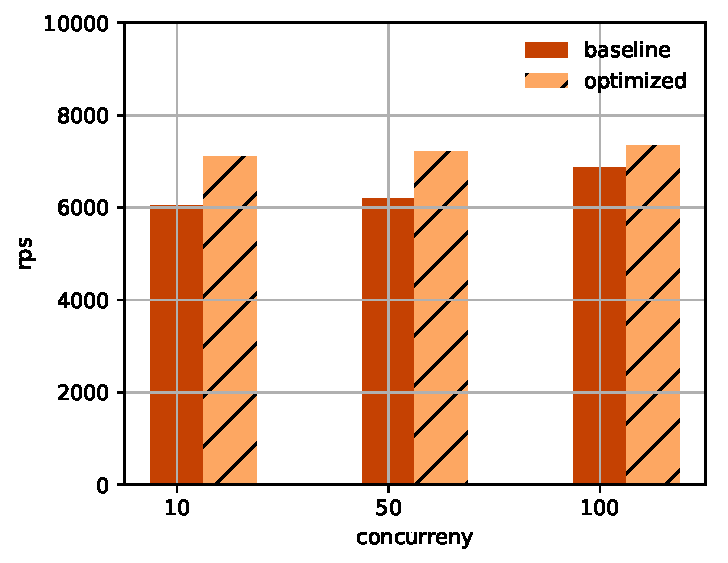
\includegraphics[width=0.70\textwidth]{ab/ab_random.pdf}
	}
\bicaption[exp:ab]{ApacheBench测试结果图 (续)}{ApacheBench测试结果图 (续)}{Fig}{ApacheBench Test Result (Con't)}
\end{figure}

ApacheBench的测试结果如图 \ref{exp:ab} 所示,深色的柱状条代表默认的随机选取策略的服务链在Apache Bench测试场景下的每秒的所能达到的累计请求完成数,浅色斜杠条纹柱代表在优化策略下测试组的测试结果。通过测试数据的整理可以发现,在线程数为10、50、100的并发请求下,优化后的服务链累计吞吐在离散分布下由3000 rps左右提升到了5000 rps左右,吞吐性能提升了60\%左右。在随机分布下由系统的吞吐的优化没有离散分布的高,但也达到了25\%左右。聚合分布下优化算法和随机策略的测试结果相近,没有提高。

这样的实验数据也是符合预期结果的。在ApacheBench这种模拟上层应用的测试下,带宽和延迟综合影响了测试的结果。首先对于离散分布而言,如图\ref{exp:ab_scattering}所示,随机策略可能会选取到性能最差的实例来组成服务链,并且这种可能性是大于如图\ref{exp:ab_random}所示的随机分布的,所以对于离散分布而言,优化的空间更大;而对于聚合分布的情况下来看,实例间并没有性能差异,所以并没有性能上的提升,其结果如图\ref{exp:ab_uniform}所示。综合来看,本设计的优化算法可以提升在离散分布和随机分布情况下模拟服务链应用的性能。
%根据实验所得数据可以看出在模拟实际应用负载下,本设计的优化系统的性能数据也是高于随机选择的。

\newpage
\section{实验小结}
本章中我们在标准通用的NUMA服务器上对本文所提出的优化系统进行了Clearwater应用性能测试和服务链通用性能测试。在实验中,我们以默认的随机资源映射策略作为参照来验证使用相同数量的物理资源的前提下,本文所提出的优化系统的有效性。本章所有实验均在三种资源分布的前提下进行了多次实验。Clearwater应用压力测试实验的结果在离散分布和随机分布下均表现出了接近40\%的延迟下降。而在网络性能测试中,本优化系统所生成的服务链相比于随机生成的服务链,在模拟服务链应用测试中分别有了15\%到30\%的延迟下降和最多接近2倍的带宽提升。在ApacheBench测试实验中,经过本系统的优化后生成的服务链可以获得25\%到60\%的吞吐提升。

需要指出的是,在聚合分布下由于某一网络功能组的功能实例均分布在同一个NUMA节点中,故具有相近的数据传输性能。在这样的前提下,本文所提出的优化算法所选取的优化决策实例与随机选取的实例没有实质性的差别,所以在无论在Clearwater应用压力测试实验还是通用的网络性能测试中均没有体现出优化效果。但是结合本章的这些实验数据,可以认为本设计的优化映射方法在大部分实际应用的场景中,确实可以有效地利用虚拟化的物理资源,提高网络服务的性能。

\section{本章小结}
本章主要介绍了基于底层感知的高性能NFV实现系统实验相关的部分内容。首先,本章介绍了实验所采用的软硬件平台,包括物理机的配置、虚拟化环境的和Clearwater平台的配置,引入了不同实例分布情况的分类说明。其次,本章对优化前后的系统进行了Clearwater应用的压力测试和网络性能测试的对比实验。压力测试用的是Clearwater提供的压力测试脚本工具,网络性能测试使用的工具包括Ping、iPerf、ApacheBench三种。压力测试所涵盖的性能测试主要包括请求的响应时间,网络测试所涵盖的性能点主要包括网络I/O的吞吐率、网络响应速率和网络的带宽。

从实验结果来看,本文所提出的优化算法在离散分布和随机分布下都体现出了一定的性能提升。无论是需要低延迟的应用(Ping实验)还是高吞吐的应用(ApacheBench实验),本算法可以有效的提高其使用相同数量物理资源下的性能收益。但是聚合分布下的分析和实验结果来看,由于资源分布本身所导致的数据传输性能限制,本设计算法并不能提高资源的使用效率。